\documentclass[11pt]{article}
% DOCUMENT COOKBOOK / SHARED SETUP. INPUT THIS FILE; DO NOT COMPILE IT.
% The ordinary document remains flowing text. Every optional feature below
% stays inactive unless explicitly used in a document or recipe.

% FOUNDATION 01: PAGE GEOMETRY AND TYPOGRAPHY (edit existing values)
% Keep a normal, flowing research manuscript. Free positioning is opt-in.
\usepackage[T1]{fontenc}
\usepackage{lmodern,microtype}
\usepackage[letterpaper,margin=1in]{geometry} % change paper/margins here
\usepackage{setspace}
\setlength{\parindent}{1.3em}
\setlength{\parskip}{0pt}

% FOUNDATION 02: SCIENTIFIC CONTENT AND COLORS
% Named palette: customize once, and every command using that color changes.
% In the document body use \color{Ink} etc. For section styling use titlesec.
% Recipe 32: mathematical symbols. amssymb loads amsfonts (\mathbb, \mathfrak);
% amsmath supplies additional operators and delimiters; bm supplies bold math.
\usepackage{amsmath,amssymb,amsthm,bm}
% DEFAULT EQUATION NUMBERING: (1.1), (1.2), (2.1), ...
% article: reset by numbered section; report/book: reset by chapter.
% For continuous (1), (2), ... numbering in an article, comment out
% the following conditional. Starred headings do not reset the counter.
\ifcsname c@chapter\endcsname
  \numberwithin{equation}{chapter}
\else
  \numberwithin{equation}{section}
\fi
\usepackage{graphicx,caption,subcaption,wrapfig,float,placeins}
\usepackage{booktabs,tabularx,array,multicol}
\usepackage{xcolor,tikz}
\usetikzlibrary{calc,positioning}
\usepackage{titlesec}
\usepackage{fancyhdr}
\usepackage{listings}
\definecolor{CUGold}{HTML}{CFB87C}
\definecolor{Ink}{HTML}{193848}
\definecolor{Teal}{HTML}{237C89}
\definecolor{Muted}{HTML}{5E7179}
\definecolor{Soft}{HTML}{EFF5F6}
\graphicspath{{figures/}}
\captionsetup{font=small,labelfont=bf}
\lstset{basicstyle=\ttfamily\footnotesize,frame=single,breaklines=true,
  columns=fullflexible,keepspaces=true,showstringspaces=false,
  keywordstyle=\color{Teal},commentstyle=\color{Muted}}

% OPT-IN REVISION NOTES: recipe 30. The blank document shows NO notes unless
% you place \todo or \todo[inline] in its body. Source-only % TODO comments
% never appear in the PDF. For a clean submission change the package line to
% \usepackage[disable,textsize=footnotesize]{todonotes}
% Do not import todonotes a second time in the main .tex file.
\setlength{\marginparwidth}{1.90cm} % margin width fits the default 1-inch margin
\setlength{\marginparsep}{0.20cm}
\usepackage[textsize=footnotesize]{todonotes}

% FOUNDATION 03: CITATIONS AND BIBLIOGRAPHY (change OPTIONS here, not elsewhere)
% style=numeric: numbered references; style=authoryear: author-year citations.
% sorting=none: citation order; sorting=nyt: name/year/title order.
% In DOCUMENT BODY, use \nocite{*} before \printbibliography to include
% every item in references.bib, even sources not cited in the text.
% For journal articles only: \nocite{*} then \printbibliography[type=article].
% Do NOT load biblatex a second time or mix with natbib/BibTeX.
\usepackage[backend=biber,style=numeric,sorting=none]{biblatex}
\addbibresource{references.bib}
% Optional shortcuts, only if wanted:
% \newcommand{\PrintAllReferences}{\nocite{*}\printbibliography}
% \newcommand{\PrintArticlesOnly}{\nocite{*}\printbibliography[type=article]}
\usepackage{aliascnt}
\usepackage[colorlinks=true,linkcolor=Ink,citecolor=Teal,urlcolor=Teal]{hyperref}
\usepackage[noabbrev,nameinlink]{cleveref}

% MATHEMATICAL ENVIRONMENTS (recipe 18; advanced customization in 31).
% Alias counters let cleveref distinguish types while sharing numbering.
% All numbered environments share a counter, reset by numbered section.
% Optional name: \begin{definition}[Relative Entropy] ... \end{definition}
\theoremstyle{plain} % bold heading, italic body
\newtheorem{theorem}{Theorem}[section]
\newaliascnt{lemma}{theorem}
\newtheorem{lemma}[lemma]{Lemma}
\aliascntresetthe{lemma}
\crefname{lemma}{lemma}{lemmas}
\Crefname{lemma}{Lemma}{Lemmas}
\newaliascnt{proposition}{theorem}
\newtheorem{proposition}[proposition]{Proposition}
\aliascntresetthe{proposition}
\crefname{proposition}{proposition}{propositions}
\Crefname{proposition}{Proposition}{Propositions}
\newaliascnt{corollary}{theorem}
\newtheorem{corollary}[corollary]{Corollary}
\aliascntresetthe{corollary}
\crefname{corollary}{corollary}{corollaries}
\Crefname{corollary}{Corollary}{Corollaries}

\theoremstyle{definition} % bold heading, upright body
\newaliascnt{definition}{theorem}
\newtheorem{definition}[definition]{Definition}
\aliascntresetthe{definition}
\crefname{definition}{definition}{definitions}
\Crefname{definition}{Definition}{Definitions}
\newaliascnt{example}{theorem}
\newtheorem{example}[example]{Example}
\aliascntresetthe{example}
\crefname{example}{example}{examples}
\Crefname{example}{Example}{Examples}
\newaliascnt{assumption}{theorem}
\newtheorem{assumption}[assumption]{Assumption}
\aliascntresetthe{assumption}
\crefname{assumption}{assumption}{assumptions}
\Crefname{assumption}{Assumption}{Assumptions}

\theoremstyle{remark} % italic heading, upright body
\newaliascnt{remark}{theorem}
\newtheorem{remark}[remark]{Remark}
\aliascntresetthe{remark}
\crefname{remark}{remark}{remarks}
\Crefname{remark}{Remark}{Remarks}
% amsthm also provides the unnumbered proof environment automatically.
% Independent counter: replace the three definition alias/declaration lines
% (newaliascnt, newtheorem, aliascntresetthe) with the following line;
% keep the crefname/Crefname lines:
% \newtheorem{definition}{Definition}[section]
% Continuous numbering: remove [section] from the theorem declaration.
% Optional unnumbered variant (declare only if needed):
% \theoremstyle{definition}
% \newtheorem*{definitionstar}{Definition}
\theoremstyle{definition} % restore the previous default declaration style

% FOUNDATION: customize an OPTIONAL precision-placed title page.
% First fontsize argument is the font size (pt); second is baseline spacing.
\newcommand{\DocTitleFont}{\color{Ink}\fontsize{25}{31}\selectfont\bfseries}
\newcommand{\DocSubtitleFont}{\color{Muted}\fontsize{14}{20}\selectfont}
\newcommand{\DocAuthorFont}{\color{Ink}\fontsize{13}{18}\selectfont}
\newcommand{\DocAffiliationFont}{\color{Muted}\fontsize{11}{15}\selectfont}

% PAGE coordinates: X from page left, Y downward from page top (cm).
% Page objects are overlays: they occupy NO flow space; use on title pages.
% \DocPageTextAt{X}{Y}{WIDTH}{TEXT}
\newcommand{\DocPageTextAt}[4]{%
  \begin{tikzpicture}[remember picture,overlay]
    \node[anchor=north west,inner sep=0pt,outer sep=0pt]
      at ([xshift=#1cm,yshift=-#2cm]current page.north west) {%
        \begin{minipage}[t]{#3}\vspace{0pt}#4\par\end{minipage}};
  \end{tikzpicture}%
}
% \DocPageImageAt{X}{Y}{WIDTH}{FILE}
\newcommand{\DocPageImageAt}[4]{%
  \begin{tikzpicture}[remember picture,overlay]
    \node[anchor=north west,inner sep=0pt,outer sep=0pt]
      at ([xshift=#1cm,yshift=-#2cm]current page.north west)
      {\includegraphics[width=#3]{#4}};
  \end{tikzpicture}%
}

% CONTAINER-LOCAL coordinates: X right, Y down from the local TikZ origin.
% Place these ONLY within a tikzpicture (usually inside a figure/minipage).
% \DocImageAt{X}{Y}{WIDTH}{FILE}
\newcommand{\DocImageAt}[4]{%
  \node[anchor=north west,inner sep=0pt,outer sep=0pt] at (#1,-#2)
    {\includegraphics[width=#3]{#4}};%
}
% \DocTextAt{X}{Y}{WIDTH}{TEXT}
\newcommand{\DocTextAt}[4]{%
  \node[anchor=north west,inner sep=0pt,outer sep=0pt] at (#1,-#2) {%
    \begin{minipage}[t]{#3}\vspace{0pt}#4\par\end{minipage}};%
}
% \DocCanvas{WIDTH}{HEIGHT}{CONTENT}: explicit space, cm; no clipping.
\newcommand{\DocCanvas}[3]{%
  \begin{tikzpicture}[x=1cm,y=1cm]
    \useasboundingbox (0,0) rectangle (#1,-#2);
    #3
  \end{tikzpicture}%
}
% \DocAutoCanvas{CONTENT}: auto-sized bounding box; no reserved height.
\newcommand{\DocAutoCanvas}[1]{%
  \begin{tikzpicture}[x=1cm,y=1cm]
    \path (0,0);#1
  \end{tikzpicture}%
}

% OPT-IN REPEATED FOOTER. The blank document does NOT enable this.
% \DocSetFooter{LEFT}{CENTER}{RIGHT}{RULE THICKNESS}
\newcommand{\DocSetFooter}[4]{%
  \fancyhf{}\fancyfoot[L]{\footnotesize #1}
  \fancyfoot[C]{\footnotesize #2}\fancyfoot[R]{\footnotesize #3}
  \renewcommand{\headrulewidth}{0pt}%
  \renewcommand{\footrulewidth}{#4}%
  \pagestyle{fancy}%
}


\title{Analysis of Multicomponent Reactive Ion Transport Systems: A Dynamical Systems Approach}
\author{Chuan Wei Heng}
\date{\today}

\begin{document}
\maketitle

\section*{Abstract}
Draft this at the end


\tableofcontents


\section{Introduction}
Since the summer of 2026, I began my research with 
Professor Ankur Gupta’s laboratory, where I investigated the 
theoretical modeling of coupled multicomponent ion transport 
in electrolyte systems. In particular, I consider an aqueous 
electrolyte containing hydrogen ($H^+$), hydroxide ($OH^-$), 
sodium ($Na^+$), and chloride ($Cl^-$) ions.

The transport of these species is governed by diffusion and 
electromigration, with the ions coupled through the 
electrostatic potential generated by their charge 
distribution. In addition, ($H^+$) and ($OH^-$) ions undergo 
an acid–base neutralization reaction to form water ($H_2O$). 
The resulting system is described by the 
Poisson–Nernst–Planck (PNP) equations coupled to chemical 
reaction kinetics.

\subsection{Motivation of Modeling Electrolyte Transport}
Two major areas of application for this study are 
electrochemical energy storage and biological systems. 
Recent advances in energy storage technologies, 
particularly lithium-ion batteries and supercapacitors, have 
highlighted the importance of understanding ionic transport 
in electrolyte solutions. Although both technologies rely on 
the movement of charged species, their energy storage 
mechanisms differ. Supercapacitors primarily store energy 
through electrostatic charge separation at 
electrode–electrolyte interfaces, whereas lithium-ion 
batteries store energy through electrochemical reactions 
involving the transfer and intercalation of ions. During 
operation, ionic transport through the electrolyte is 
coupled to the flow of electrons through an external 
circuit, allowing stored energy to be delivered to 
electronic devices. Consequently, understanding the 
mechanisms governing ionic transport is essential to the 
modeling and optimization of these technologies.

In biological systems, coupled ionic transport plays a 
fundamental role in numerous physiological processes, 
particularly in the nervous system. The transport of sodium, 
potassium, calcium, and chloride ions across cell membranes 
governs the establishment of membrane potentials and the 
generation and propagation of electrical signals in neurons. 
These processes enable communication between neurons and are 
essential to sensory perception, muscle contraction, and 
cognitive functions. Ionic transport is also central to the 
regulation of intracellular pH, cellular volume, and 
electrolyte balance. The interplay between diffusion, 
electromigration, membrane selectivity, and biochemical 
reactions gives rise to complex transport dynamics. 
Consequently, developing a fundamental understanding of 
coupled multicomponent ion transport is also crucial in the 
modeling of biological and physiological systems.

\subsection{The Set up}

The following setup is that of a classical PDE problem 
statement, identifying an appropriate governing equation 
which describes the underlying dynamics of the system of 
interest, and prescribing suitable boundary conditions.

\subsection*{Governing Equations}

The conservation equation for each ionic species is

\begin{equation}
    \frac{\partial c_i}{\partial t}
    = -\nabla\cdot\bm{J}_i + R_i,
    \qquad
    i \in \{H^+, OH^-, Na^+, Cl^-\},
    \label{eq:continuity}
\end{equation}

where $c_i$ denotes the concentration, $\bm{J}_i$
the molar flux, and $R_i$ the net rate of production
of species $i$.

The ionic flux is described by the Nernst--Planck
equation,

\begin{equation}
    \bm{J}_i
    = -D_i\left(
        \nabla c_i
        + \frac{z_i F}{RT}c_i\nabla\phi
    \right),
    \label{eq:nernst_planck}
\end{equation}

where $D_i$ and $z_i$ are the diffusivity and valence
of species $i$, respectively. Furthermore, $F$ is
Faraday's constant, $R$ is the ideal gas constant,
$T$ is the absolute temperature, and $\phi$ is the
electrostatic potential.

The acid--base reaction is modeled using the
following second-order reaction kinetics:

\begin{equation}
    \begin{aligned}
        R_{H^+} = R_{OH^-}
        &= -kc_{H^+}c_{OH^-},\\
        R_{Na^+} = R_{Cl^-}
        &= 0.
    \end{aligned}
    \label{eq:reaction}
\end{equation}

Finally, the electrostatic potential is determined
self-consistently through Poisson's equation,

\begin{equation}
    -\varepsilon\nabla^2\phi
    = \rho_e
    = F\sum_i z_i c_i,
    \label{eq:poisson}
\end{equation}

where $\varepsilon$ denotes the permittivity
and $\rho_e$ is the local charge density.

\subsection*{Domain and Boundary Conditions}

We consider a one-dimensional domain of length $L$,
with prescribed ionic concentrations and electrostatic
potentials at both boundaries.

\begin{figure}[htbp]
    \centering
    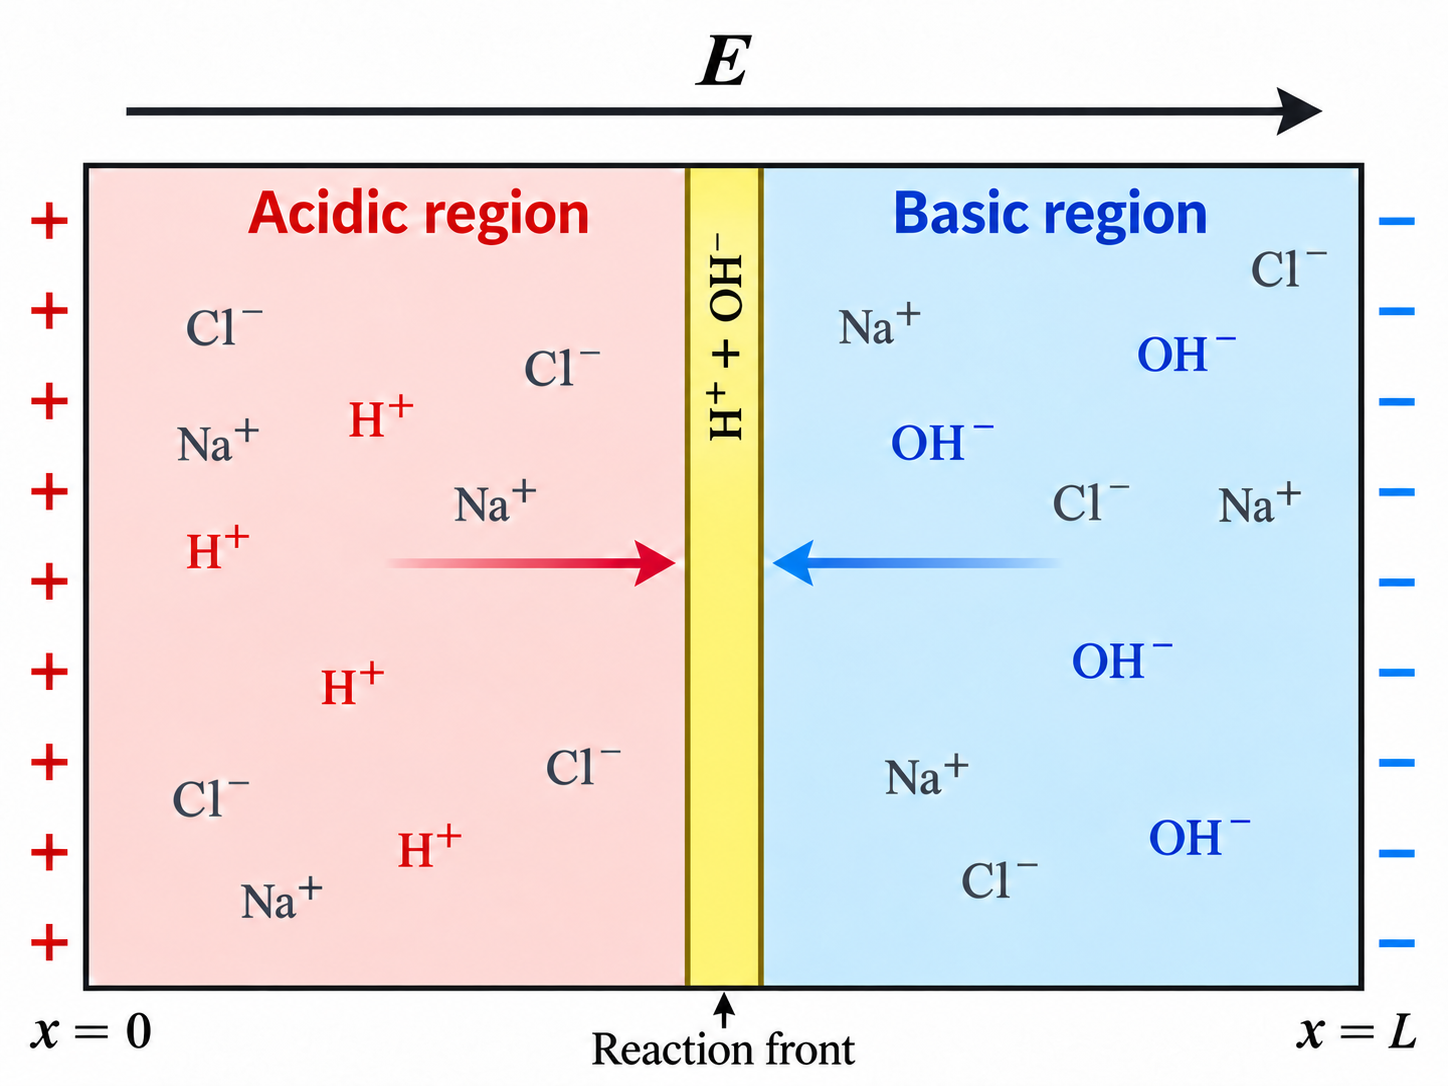
\includegraphics[width=0.65\textwidth]
        {figures/Electrochemical Reaction Front Diagram.png}
    \caption{Schematic of the one-dimensional
    electrolyte domain and acid--base reaction front.}
    \label{fig:reaction_front_domain}
\end{figure}

At the left boundary, $x=0$,

\begin{equation}
    \begin{aligned}
        c_{H^+} &= c_0,
        &\qquad c_{Na^+} &= c_s,\\
        c_{OH^-} &= 0,
        &\qquad c_{Cl^-} &= c_0+c_s,\\
        \phi &= \phi_0.
    \end{aligned}
    \label{eq:bc_left}
\end{equation}

At the right boundary, $x=L$,

\begin{equation}
    \begin{aligned}
        c_{H^+} &= 0,
        &\qquad c_{Cl^-} &= 0,\\
        c_{Na^+} &= c_0,
        &\qquad c_{OH^-} &= c_0,\\
        \phi &= \phi_L.
    \end{aligned}
    \label{eq:bc_right}
\end{equation}

The initial ionic concentrations in the interior
of the domain are prescribed as

\begin{equation}
    c_i(x,0)=0,
    \qquad 0<x<L,
    \qquad \forall i.
    \label{eq:initial}
\end{equation}

\subsection{A Recent Development: Electroconvective Instabilities}

Our recent research has led us to hypothesize that
electroconvective vortices may develop near an acid--base
reaction front under an externally applied electric
potential. This hypothesis is motivated by earlier work
on electroconvective instabilities near ion-selective
membranes, particularly the work of
\textcite{rubinstein2000electro}.

In these systems, electrokinetic instabilities can
generate vortical fluid motion near the membrane
interface. This phenomenon is commonly associated
with the Rubinstein--Zaltzman instability.

\begin{figure}[htbp]
    \centering
    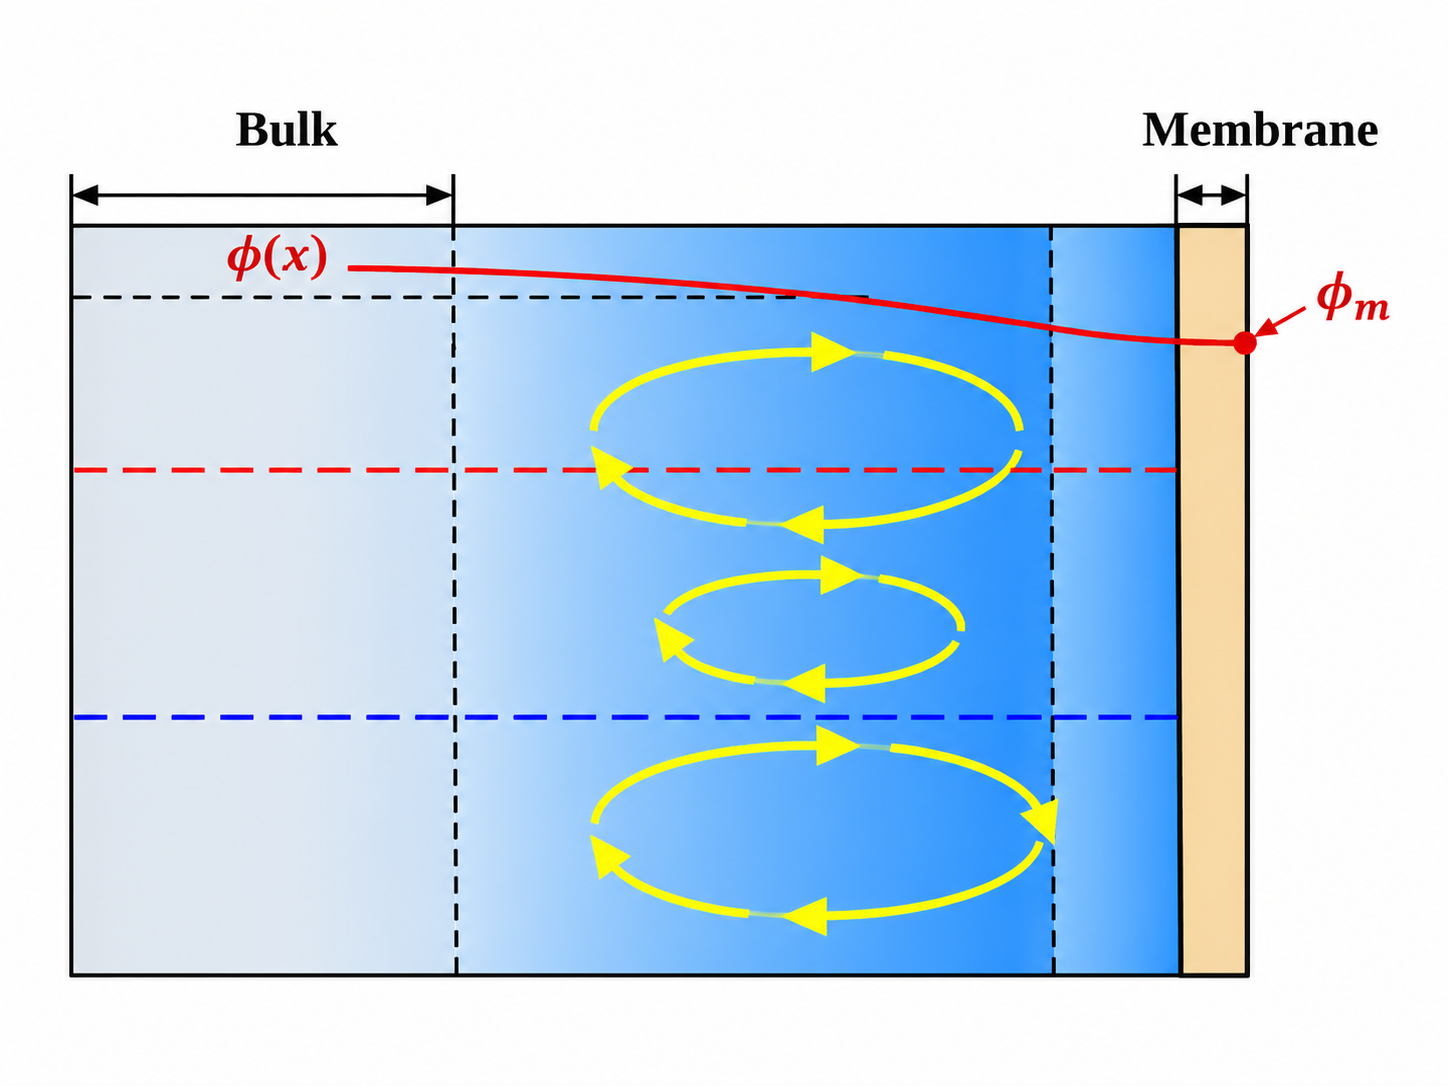
\includegraphics[width=0.55\textwidth]
        {figures/membrane_vortex.png}
    \caption{Schematic of electroconvective vortices
    near the interface of an ion-selective membrane.}
    \label{fig:membrane_vortices}
\end{figure}

Inspired by this mechanism, we seek to investigate
whether a related instability can arise in a
membraneless electrolyte system, where the acid--base
reaction front creates spatial variations in ionic
concentrations and electrical properties.

Unlike membrane-based systems, the proposed instability
would occur without a physical ion-selective interface.
Consequently, the existence and underlying mechanism
of such an instability remain to be established.

Our central research question is therefore:
\textit{Can a Rubinstein--Zaltzman-type electroconvective
instability arise near a membraneless acid--base
reaction front?}

\begin{figure}[H]
    \centering
    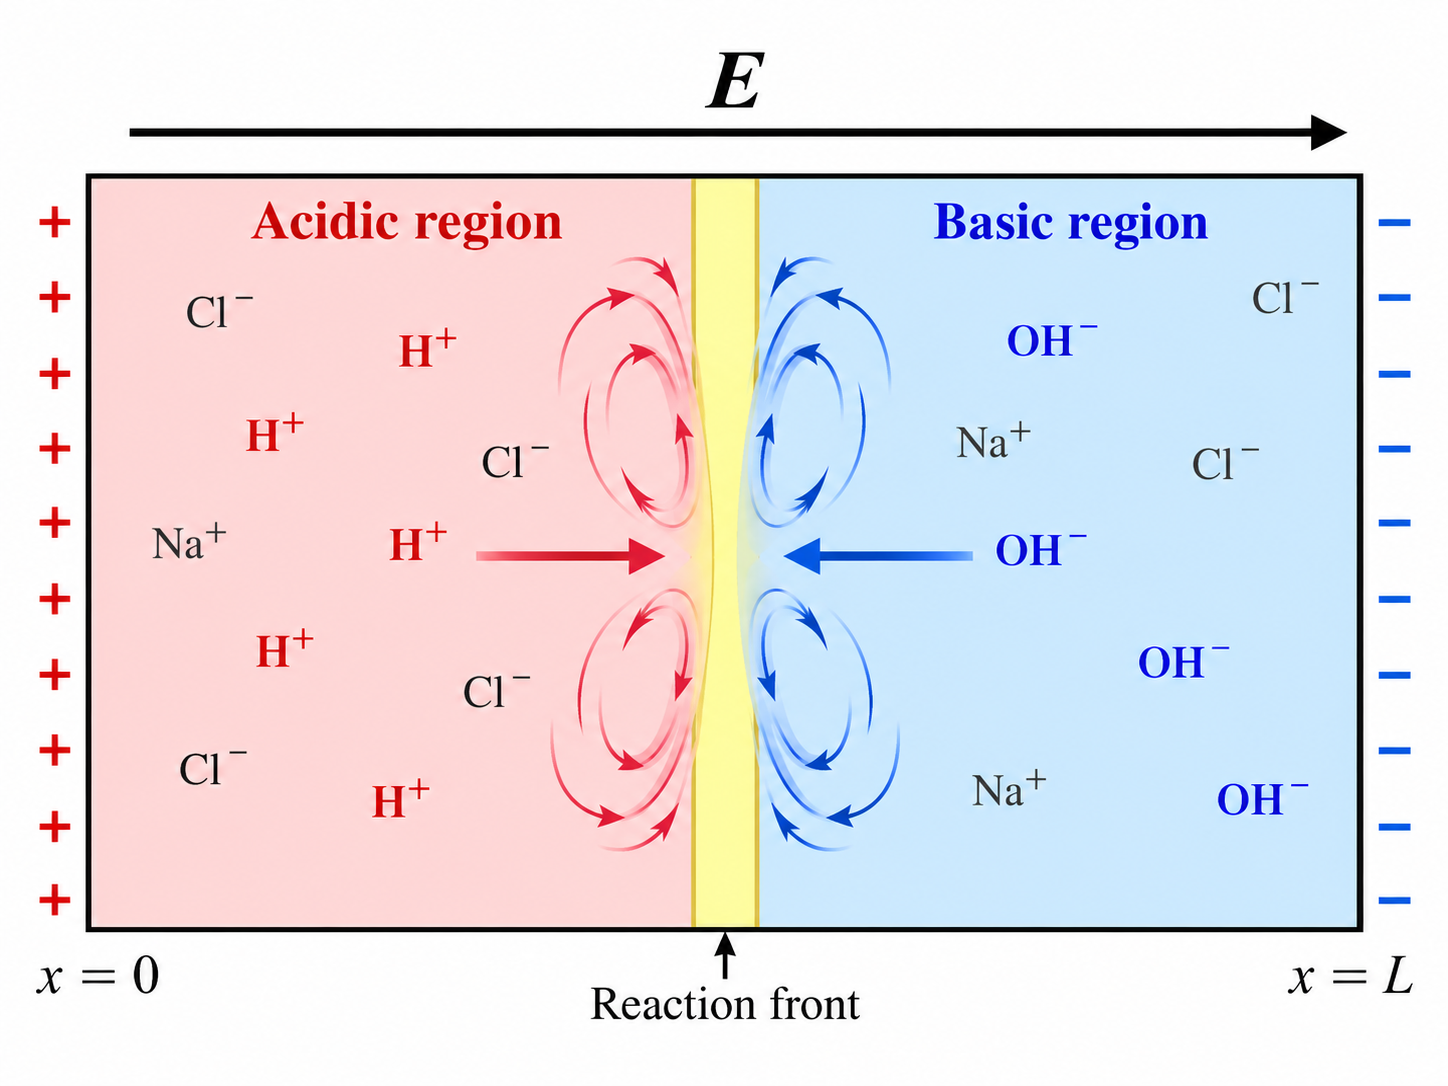
\includegraphics[width=0.55\textwidth]
        {figures/membraneless_vortex.png}
    \caption{Schematic of hypothesized electroconvective
    vortices near a membraneless acid--base reaction
    front under an applied electric potential.}
    \label{fig:membraneless_vortices}
\end{figure}

\FloatBarrier

\subsection{Existing Work}

\subsubsection{Nondimensionalization}

Dropping the hats, our nondimensionlized PNP system is

\begin{equation}
    \frac{\partial c_i}{\partial t}
    = -\nabla\cdot\bm{J}_i + R_i,
    \label{eq:nondim_continuity}
\end{equation}

\begin{equation}
    \bm{J}_i
    = -d_i\left(
        \nabla c_i
        + z_ic_i\nabla\phi
    \right),
    \label{eq:nondim_nernst_planck}
\end{equation}

\begin{equation}
    \begin{aligned}
        R_{H^+} = R_{OH^-}
        &= -Dac_{H^+}c_{OH^-},\\
        R_{Na^+} = R_{Cl^-}
        &= 0.
    \end{aligned}
    \label{eq:reaction}
\end{equation}

\begin{equation}
    -\kappa^2\nabla^2\phi
    = \sum_i z_i c_i.
    \label{eq:nondim_poisson}
\end{equation}

\subsubsection{Electroneutrallity and Zero-Current Assumption}

\subsubsection{1D Steady State Semianalytic ENP Solution}

\subsubsection{Numerical ENP Solutions}

\subsubsection{Numerical PNP Solutions}


\subsection{Connection to Dynamical Systems}

The application of dynamical systems theory to
electrokinetic transport has been demonstrated in
several previous studies. The pioneering work of
\textcite{rubinstein2000electro} established a
theoretical framework for understanding the onset
of electroconvective instability near permselective
membranes. Subsequent investigations have explored
the nonlinear dynamics of these systems, including
transitions between distinct dynamical regimes and
the emergence of chaotic motion
\parencite{davidson2016dynamical,demekhin2013direct}.

Beyond membrane-based systems, electrohydrodynamic
instabilities have also been investigated in
electrolytes exhibiting spatial variations in
electrical conductivity. In particular,
\textcite{sharan2017mechanism} investigated the
mechanisms governing instability in systems with
collinear conductivity gradients and electric
fields, while \textcite{oddy2005multiple} extended
the investigation of electrokinetic instabilities
to multicomponent ionic transport systems.

Inspired by these studies, our broader research
seeks to extend the investigation of electrokinetic
instabilities to a membraneless system in which
spatial variations in ionic concentrations and
electrical conductivity arise through chemical
reaction. To the best of our knowledge, the
stability and bifurcation characteristics of the
particular multicomponent reactive transport
configuration considered in this study remain
largely unexplored.

The mathematical investigation of this system
presents a considerable challenge. Unlike the
finite-dimensional ODE systems traditionally
considered in classical dynamical systems theory,
the system of interest is governed by a set of
nonlinear, coupled PDEs, with spatially nonuniform
stationary solutions and multiple interacting
physical mechanisms. Consequently, the direct
application of classical dynamical systems
techniques requires substantial mathematical
extensions to accommodate the infinite-dimensional
nature of the system.

Given the complexity and exploratory nature of
this research problem, the present project serves
as a preliminary investigation into the proposed
electroconvective instability. We restrict our
attention to the one-dimensional
PNP system coupled to chemical
reaction kinetics, investigating the stability
and potential bifurcations of stationary solutions
without incorporating fluid motion.

This project constitutes an initial step toward
addressing a considerably more complex research
problem involving higher-dimensional ionic
transport coupled to fluid motion.


\section{Methods}

\subsection{From ODEs to PDEs}

Much of classical dynamical systems theory is concerned
with the analysis of finite-dimensional systems governed
by ordinary differential equations (ODEs). Consider an
arbitrary autonomous dynamical system of the form

\begin{equation}
    \frac{d\bm{u}}{dt}
    = \bm{f}(\bm{u};\mu),
    \qquad \bm{u}\in\mathbb{R}^n,
\end{equation}

where $\mu$ denotes a control parameter. An equilibrium
solution $\bm{u}^*$ satisfies

\begin{equation}
    \bm{f}(\bm{u}^*;\mu)=\bm{0}.
\end{equation}

The local stability of this equilibrium may be
investigated by introducing a small perturbation,

\begin{equation}
    \bm{u}(t)=\bm{u}^*+\epsilon\bm{v}(t),
    \qquad 0<\epsilon\ll 1.
\end{equation}

Substitution into the governing equation and a
first-order Taylor expansion about the equilibrium
yield the linearized system

\begin{equation}
    \frac{d\bm{v}}{dt}
    =\bm{J}(\bm{u}^*;\mu)\bm{v},
\end{equation}

where $\bm{J}$ is the Jacobian matrix of $\bm{f}$
evaluated at the equilibrium. Assuming a perturbation
of the form $\bm{v}(t)=\bm{w}e^{\lambda t}$ yields
the eigenvalue problem

\begin{equation}
    \bm{J}\bm{w}=\lambda\bm{w}.
\end{equation}

The stability of the equilibrium may then be
characterized through the eigenvalues of the Jacobian.
In particular, if all eigenvalues have strictly negative
real parts, the equilibrium is locally asymptotically
stable, whereas the existence of an eigenvalue with
a positive real part implies instability. Furthermore,
by investigating how these eigenvalues vary with the
control parameter $\mu$, one may identify potential
bifurcation points.

\medskip

The system considered in this study, however, is
governed by partial differential equations (PDEs).
Unlike an ODE system, whose state is represented by
a finite-dimensional vector, the state of a PDE
system is represented by a spatially distributed
function. Consequently, the problem is extended from
a finite-dimensional to an infinite-dimensional
dynamical system.

Consider an arbitrary autonomous evolution PDE
of the form

\begin{equation}
    \frac{\partial\bm{u}}{\partial t}
    =\mathcal{F}[\bm{u};\mu],
    \qquad \bm{x}\in\Omega,
\end{equation}

where $\mathcal{F}$ denotes a potentially nonlinear
differential operator and $\Omega$ is the spatial
domain. A stationary solution $\bm{u}^*(\bm{x})$
satisfies

\begin{equation}
    \mathcal{F}[\bm{u}^*;\mu]=\bm{0},
\end{equation}

together with the prescribed boundary conditions.
Analogous to the ODE formulation, a small perturbation
is introduced as

\begin{equation}
    \bm{u}(\bm{x},t)
    =\bm{u}^*(\bm{x})+\epsilon\bm{v}(\bm{x},t).
\end{equation}

Linearization about the stationary solution yields

\begin{equation}
    \frac{\partial\bm{v}}{\partial t}
    =\mathcal{L}\bm{v},
    \qquad
    \mathcal{L}=D_{\bm{u}}\mathcal{F}[\bm{u}^*;\mu],
\end{equation}

where $\mathcal{L}$ is the linearized differential
operator, serving as the infinite-dimensional
analogue of the Jacobian matrix. Assuming a
perturbation of the form

\begin{equation}
    \bm{v}(\bm{x},t)
    =\bm{w}(\bm{x})e^{\lambda t},
\end{equation}

yields the differential eigenvalue problem

\begin{equation}
    \mathcal{L}\bm{w}=\lambda\bm{w},
\end{equation}

subject to the appropriate perturbation boundary
conditions. The stability investigation therefore
transitions from the analysis of the eigenvalues
of a finite-dimensional matrix to the analysis
of the spectrum of a differential operator.

Furthermore, analogous to the finite-dimensional
formulation, bifurcation theory may be extended
to investigate qualitative changes in stationary
solutions and their stability as control parameters
vary.

The methodology employed in this study is therefore
largely inspired by classical ODE-based dynamical
systems theory, with the necessary extensions to
accommodate spatial dependence, differential
operators, and boundary conditions. In particular,
linearization, spectral stability analysis, and
bifurcation theory are employed to investigate
the dynamics of the coupled ionic transport system.
Numerical methods are subsequently utilized where
analytical solutions become intractable.


\subsection{Stationary Solutions}

\subsection{Stability Analysis}

Recall our system given by \eqref{eq:nondim_continuity}, 
\eqref{eq:nondim_nernst_planck}, and \eqref{eq:nondim_poisson}. We seek a 
stationary solution denoted by $c^*_i(x)$, and $\phi^*(x).$
By definition, $\frac{\partial c^*_i}{\partial t}=0.$ 
Restricting ourselves to one spatial dimension,
the governing equations reduce to

\begin{equation}
    0=-\frac{dJ_i^*}{dx}+R_i^*,
    \label{eq:steady_continuity}
\end{equation}

\begin{equation}
    J_i^*
    =-d_i\left(
        \frac{dc_i^*}{dx}
        +z_ic_i^*\frac{d\phi^*}{dx}
    \right),
    \label{eq:steady_nernst_planck}
\end{equation}

\begin{equation}
    \begin{aligned}
        R_{H^+}^*=R_{OH^-}^*
        &=-\mathrm{Da}\,c_{H^+}^*c_{OH^-}^*,\\
        R_{Na^+}^*=R_{Cl^-}^*&=0.
    \end{aligned}
    \label{eq:steady_reaction}
\end{equation}

\begin{equation}
    -\kappa^2\frac{d^2\phi^*}{dx^2}
    =\sum_i z_i c_i^*,
    \label{eq:steady_poisson}
\end{equation}

subject to the nondimensionalized Dirichlet
boundary conditions. Together, these equations
constitute a coupled nonlinear boundary-value
problem.

Substituting \eqref{eq:steady_nernst_planck}
into \eqref{eq:steady_continuity} yields

\begin{equation}
    0=d_i\frac{d}{dx}\left(
        \frac{dc_i^*}{dx}
        +z_ic_i^*\frac{d\phi^*}{dx}
    \right)+R_i^*.
    \label{eq:steady_pnp}
\end{equation}




\subsubsection{Linearization of the Governing Equations}

\subsubsection{Spectral Stability Analysis}

\subsection{Bifurcation Analysis}

\subsection{Numerical Investigation}


\section{Results and Discussion}

\section{Conclusion}

\section*{AI Disclosure and Usage}
Assistance in writing

Assistance in learning difficult content fast

Assistance in literature review

ODE to PDE section was largely AI generated with careful 
vetting.

% OPTIONAL bibliography (uncomment ONE option):
\printbibliography              % Only cited entries
% \nocite{*}\printbibliography   % ALL bibliography entries, even uncited
% \nocite{*}\printbibliography[type=article] % ALL articles only
\end{document}
